\begin{frame}[allowframebreaks]{Autoencoders: Applications}
\textbf{Dimensionality Reduction}

Autoencoders are widely used as nonlinear alternatives to traditional dimensionality reduction techniques like PCA (Principal Component Analysis).
\begin{itemize}
    \item The encoder compresses high-dimensional data into a low-dimensional latent space.
    \item This latent representation preserves meaningful features and patterns.
    \item Especially effective for visualizing data or preprocessing inputs for downstream tasks.
\end{itemize}
\textbf{Use Case}: Visualizing high-dimensional datasets (e.g., MNIST) in 2D or 3D.

\framebreak

\begin{figure}
    \centering
    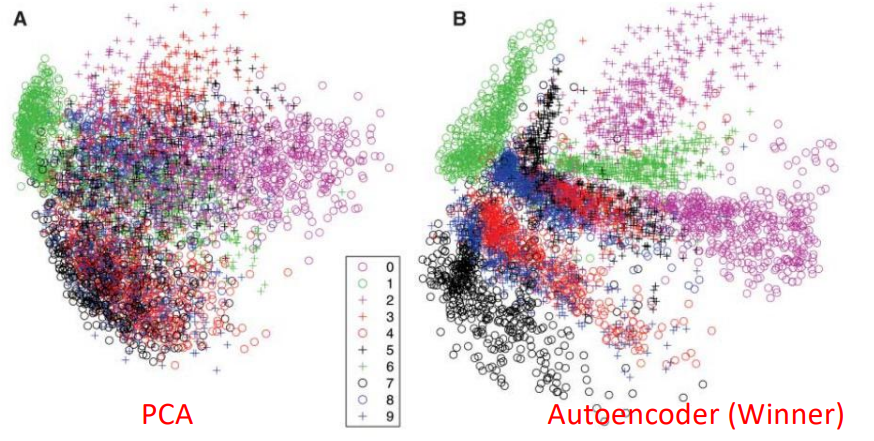
\includegraphics[height=0.8\textheight, width=\textwidth, keepaspectratio]{images/autoencoder/image_representation.PNG}
    \caption{t-SNE visualization on MNIST digits dataset. PCA vs. Autoencoders. The image vector is projected into $\mathbb{R}^2$.}
\end{figure}

\framebreak

\textbf{Super-Resolution}

Autoencoders can be used to reconstruct high-resolution images from their low-resolution counterparts.

\begin{itemize}
    \item Input: Low-resolution image.
    \item Output: High-resolution image.
    \item Often implemented with convolutional layers for spatial pattern learning.
\end{itemize}
\textbf{Use Case}: Enhancing medical images, satellite images, or upscaling low-resolution photos.

\framebreak

\begin{figure}
    \centering
    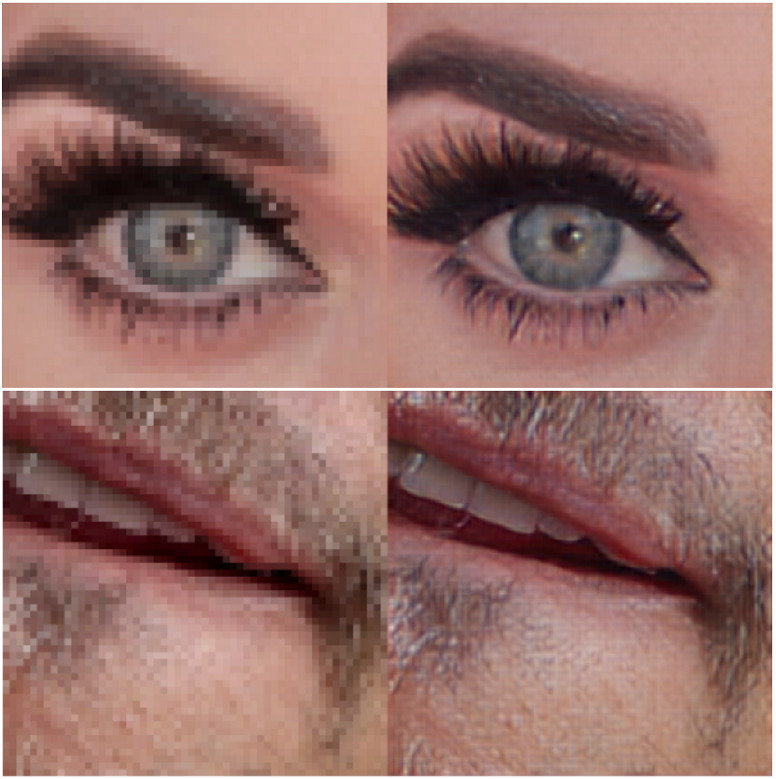
\includegraphics[height=0.8\textheight, width=\textwidth, keepaspectratio]{./images/autoencoder/image_enhancement.png}
    \caption{Image super-resolution using Autoencoders}
\end{figure}

\framebreak

\textbf{Image Colorization}

Autoencoders can learn to predict color information for grayscale images.

\begin{itemize}
    \item Input: Grayscale image (1 channel).
    \item Output: Colorized image (3 channels — RGB).
    \item Requires learning semantic and contextual relationships to apply realistic colors.
\end{itemize}
\textbf{Use Case}: Restoring historical black-and-white photos.

\framebreak

\begin{figure}
    \centering
    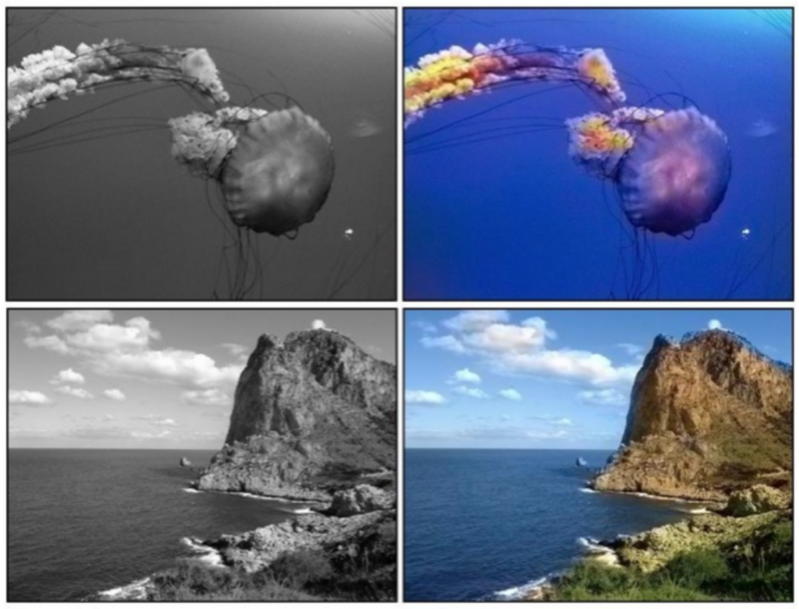
\includegraphics[height=0.8\textheight, width=\textwidth, keepaspectratio]{./images/autoencoder/image_colorization.png}
    \caption{Image colorization using Autoencoders}
\end{figure}

\end{frame}